\documentclass[a4paper]{article}
%% Packages
\usepackage[dvipdfmx, hidelinks]{hyperref}
\usepackage[dvipdfmx]{graphicx}

\usepackage{epstopdf}

\usepackage{tcolorbox}
\usepackage{listings}
\lstset{%
  language={Java},%
  basicstyle = \scriptsize\ttfamily,
  breaklines = true,
  breakindent = 40pt,
  numbers=left,
  numberstyle = {\tiny \emph},
  frame = tlRB,
  frameround = ffft,
  framesep = 3pt,
  rulesep = 1pt,
  rulecolor = {\color{blue}},
  rulesepcolor = {\color{blue}},
  flexiblecolumns = true,
  keepspaces = false,
  identifierstyle = \itshape\scriptsize,
  commentstyle = \fontfamily{ptm}\selectfont\scriptsize\color{red},
  stringstyle = \scshape\scriptsize,
  tabsize = 2,
}

\oddsidemargin -5.4mm
\evensidemargin -5.4mm
\textwidth 170mm
\topmargin -5.4mm
\headheight 0pt
\headsep 0pt
\textheight 257mm
\usepackage{ascmac}
%%
\begin{document}
%%
\title{RoboCup Rescue Simulator and Agent Development Framework Manual}
\date{October 14, 2018}
%%
\maketitle
%%
\tableofcontents
%%
\section{Introduction}
The purpose of this manual is to facilitate the understanding of the first contact with the RoboCup Rescue Simulation server and to help people interested in participating in RoboCup Rescue Agent Simulation competitions.
%%
\section{Installation}
This manual assumes the simulator and agents will run in a Linux machine even though it is possible to run them in Microsoft Windows or Apple macOS. We recommend to use Linux because it is open-source and most of the distributions have a good support from the users' community. If you have never used Linux before and intend to, we recommend starting with a user-friendly distribution, such as Ubuntu\footnote{\url{https://www.ubuntu.com/}} or Fedora\footnote{\url{https://getfedora.org}}.
%%
\subsection{Software Requirements}
%%
\begin{itemize}
  \item Java OpenJDK 8+\footnote{\url{https://openjdk.java.net/}}
  \item Git
  \item Gradle
  \item Utilities like \emph{wget}, \emph{bash}, \emph{xterm}, \emph{tar}, \emph{gzip}, etc.\\
        If you are using Ubuntu, all of these software are present in the
        default software repositories.
\end{itemize}
%%
%%
\subsection{Installing RoboCup Rescue Simulation (RCRS) Server}
\begin{enumerate}
 \item Clone the simulation server from
       \url{https://github.com/roborescue/rcrs-server}.
 \item Change to the directory ``rcrs-server''.
       \begin{enumerate}
	\item If you use macOS, patch the file ``boot/functions.sh''
	      like\\

	      ``\verb|sed -i -e "/readlink/s/^/#/" boot/functions.sh|''.
       \end{enumerate}
 \item Compile the simulator using the commands \texttt{gradle clean}
       and \texttt{gradle completeBuild}.       
 \item Check the message at the end of the installation.
       If the installation is successfully completed, you get the message ``BUILD SUCCESSFUL''; otherwise you get ``BUILD FAILED''.
\end{enumerate}

If you are using Ubuntu, the installation proceeds according to the commands below:

\begin{center}
  \begin{tcolorbox}[title=Installation on Ubuntu, width=.98\linewidth]
  {\ttfamily\small
  \$ git clone https://github.com/roborescue/rcrs-server.git\\
   \$ cd rcrs-server\\
   (\$ sed -i -e \verb|"/readlink/s/^/#/"| boot/functions.sh \# Only required for macOS)\\
  \$ gradle clean\\
  \$ gradle completeBuild
  }
  \end{tcolorbox}
\end{center}

The following message will be appeared if the installation is successfully completed.

\begin{center}
  \begin{tcolorbox}[title=Install Completion, width=.98\linewidth]
  {\ttfamily
  BUILD SUCCESSFUL in 2s\\
  1 actionable task: 1 executed
  }
  \end{tcolorbox}
\end{center}
%%
\subsection{Compiling the Agent Development Framework (ADF) Sample Agents}
%%
Download the sample agents with ADF by cloning the \url{https://github.com/roborescue/rcrs-adf-sample.git} repository. Then, you move to \texttt{rcrs-adf-sample} directory and compile the sample agents using the
script \texttt{compile.sh}.

If you are using Ubuntu, you can get and compile the ADF with the following commands:

\begin{center}
  \begin{tcolorbox}[title=Download ADF on Ubuntu, width=.98\linewidth]
  {\ttfamily\small
  \$ git clone https://github.com/roborescue/rcrs-adf-sample.git\\
  \$ cd rcrs-adf-sample\\
   \$ ./compile.sh
   % Old \$ java -jar ./library/rescue/adf/adf-core.jar -compile\\
  }
  \end{tcolorbox}
\end{center}
%%
\section{Running the ADF Sample Agents on RCRS Server}
%%
\subsection{Running without Precomputation}
%%
To run the sample agents, you must open two terminal windows. One is used to run the simulation server (i.e., the simulator) and the other is used to run the agents.
%%
\subsubsection{Running the Simulation Server}
%%
Use one terminal window and move to the boot directory inside the simulator's folder (\texttt{rcrs-server}). Then, type \texttt{bash start-comprun.sh}. The sequence of commands are:

\begin{center}
   \begin{tcolorbox}[title=Running Simulation Server, width=.98\linewidth]
    {\ttfamily
    \$ cd rcrs-server\\
    \$ cd boot\\
    \$ bash start-comprun.sh
    }
  \end{tcolorbox}
\end{center}

When the simulation server runs correctly, the window in Fig. \ref{fig:simulator01} will appear.

\begin{figure}[h]
 \begin{center}
  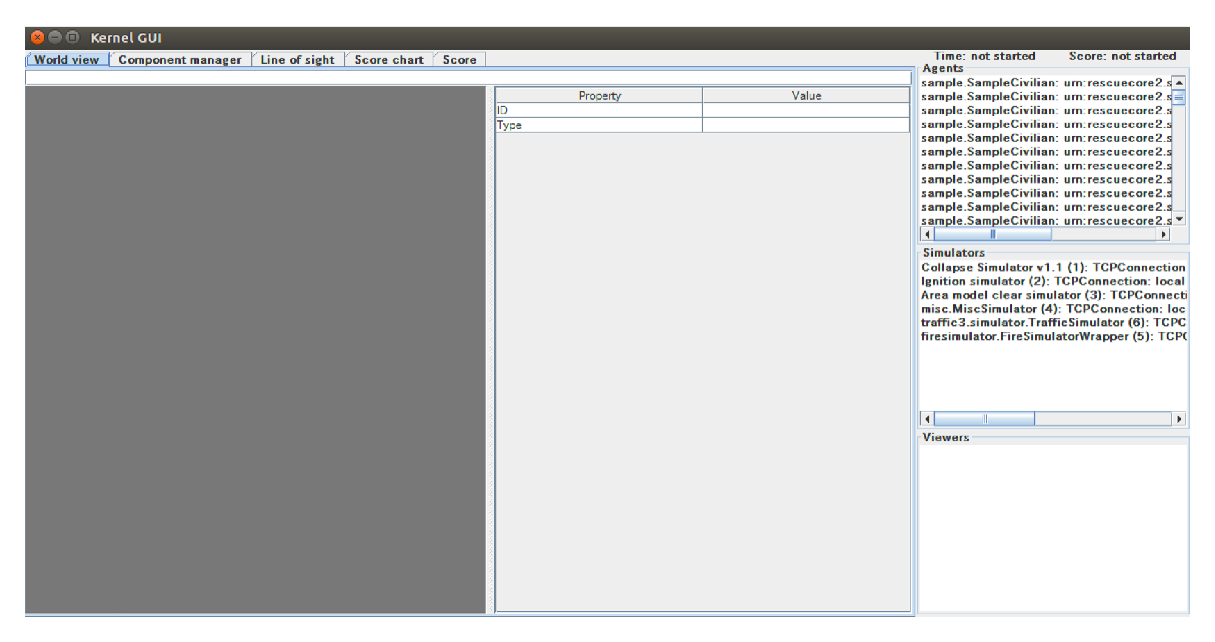
\includegraphics[width=.9\linewidth]{figs/simulator01.eps}
  \caption{Running the Simulation Server}
  \label{fig:simulator01}
 \end{center}
\end{figure}
%%
%%
\subsubsection{Running the ADF Sample Agents}
%%
After running the simulation server, move to \texttt{rcrs-adf-sample} directory on the other terminal window and run the agents by the following commands:

\begin{center}
   \begin{tcolorbox}[title=Running Sample Agents, width=.98\linewidth]
    {\ttfamily
    \$ sh launch.sh -all\\
    $[$FINISH$]$ Done connecting to server (3 agents)
    }
  \end{tcolorbox}
\end{center}

If the agents can connect with the simulator, the state of the agents and a city are shown on the left-hand side in the window shown in Fig. \ref{fig:simulator01}. Then, the simulation is started as shown in Fig. \ref{fig:simulator02}.

\begin{figure}[h]
 \begin{center}
  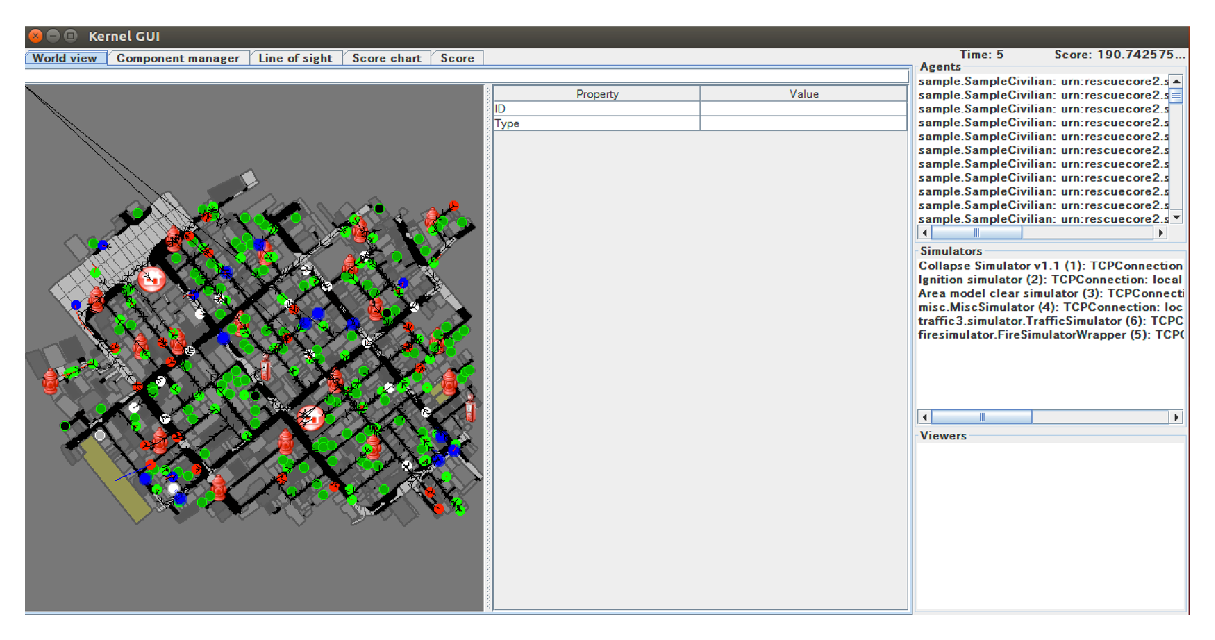
\includegraphics[width=1.0\linewidth]{figs/simulator02.eps}
  \caption{Starting the Simulation}
  \label{fig:simulator02}
 \end{center}
\end{figure}
%%
%%
\subsection{Running with Precomputation}
%%
Agents can examine a simulation scenario by performing a precomputation of it before starting the simulation. The length of the precomputation is predefined to 2 minutes in the competition. The precomputation needs two terminal windows likewise.
%%
\subsubsection{Running the Simulation Server for Precomputation}
%%
Use one terminal window and move to the boot directory inside the simulator's folder (\texttt{rcrs-server}). Then, type \texttt{bash start-precompute.sh}. These commands are:

\begin{center}
   \begin{tcolorbox}[title=Running Simulation Server, width=.98\linewidth]
    {\ttfamily
    \$ cd rcrs-server\\
    \$ cd boot\\
    \$ bash start-precompute.sh
    }
  \end{tcolorbox}
\end{center}
%%
%%
\subsubsection{Running the ADF Sample Agents for Precomputation}
%%
After running the simulation server for the precomputation, move to the ADF directory on the other terminal window and run the agents executing the commands:

\begin{center}
   \begin{tcolorbox}[title=Running Sample Agents, width=.98\linewidth]
    {\ttfamily
    \$ sh launch.sh -t 1,0,1,0,1,0 -h localhost -pre 1 \& APID=\$! ; sleep 120 ;
    kill \$APID\\
    $[$START $]$ Connect to server (host:localhost, port:7000)\\
    $[$INFO  $]$ Connected - adf.agent.platoon.PlatoonFire@756ec19c (PRECOMPUTATION)\\
    $[$INFO  $]$ Connected - adf.agent.platoon.PlatoonPolice@366bbbe (PRECOMPUTATION)\\
    $[$INFO  $]$ Connected - adf.agent.platoon.PlatoonAmbulance@2a453513 (PRECOMPUTATION)\\
    ********************\\
    $[$FINISH$]$ Connect PoliceForce (success:1)\\
    $[$FINISH$]$ Connect AmbulanceTeam (success:1)\\
    $[$FINISH$]$ Connect FireBrigade (success:1)\\
    $[$FINISH$]$ Done connecting to server (3 agents)
    }
  \end{tcolorbox}
\end{center}
%%
%%
\subsubsection{Running the Simulation}
%%
When the precomputation is completed, push \texttt{Control-C} and type \texttt{sh kill.sh} to stop the simulation server of running. Then, type \texttt{bash start-comprun.sh} to start the simulation server again to run the simulation scenario. The commands are:

\begin{center}
   \begin{tcolorbox}[title=Running Simulation Server, width=.98\linewidth]
    {\ttfamily
    Control-C\\
    \$ sh kill.sh\\
    \$ bash start-comprun.sh
    }
  \end{tcolorbox}
\end{center}

\subsubsection{Running the ADF Sample Agents}
After running the simulation server, move to the ADF directory on the other terminal window and run the agents using the commands:

\begin{center}
   \begin{tcolorbox}[title=Running Sample Agents, width=.98\linewidth]
    {\ttfamily
    \$ sh lauch.sh -all\\
    $[$FINISH$]$ Done connecting to server (3 agents)
    }
  \end{tcolorbox}
\end{center}

\section{Simulation Server Options}
\subsection{Directories}
Important directories of the simulation server are:
\begin{itemize}
 \item boot/: scripts to run the simulation server
       \begin{itemize}
	 \item boot/config/: configuration files of the simulation server.
	\item boot/logs/: log files.
       \end{itemize}
 \item build/: the simulation server's Java classes.
 \item jars/: the simulation server's JAR files.
 \item lib/: libraries used by the simulation server.
 \item maps/: maps that can be ran in the simulation server.
 \item modules/: the simulation server's source code.
 \item oldsims/: source code of some of the simulation server's older versions.
\end{itemize}
%%
%%
\subsection{Parameters}
%%
The following parameters can be used to run the simulation server:
%%
\begin{itemize}
 \item -m MAPDIR or {-}{-}map MAPDIR, where MAPDIR is the path to the directory containing the map you want to run (default is ../maps/gml/Kobe2013/map).
 \item -c CONFIGDIR or {-}{-}config CONFIGDIR, where CONFIGDIR is the directory containing the configuration associated with a map (default is ./config).
 \item -l LOGDIR or {-}{-}log LOGDIR, where LOGDIR is the directory where the log files will be stored (default is ./logs).
\end{itemize}
%%

These parameters can be used at running a precomputaion and a simulation. You must use the same parameters regarding MAPDIR and CONFIGDIR to run a simulation server with or without precomputation. An example of how to run the simulation server using these parameters is:
%%
\begin{center}
   \begin{tcolorbox}[title=Running Simulation Server with Options, width=.98\linewidth]
    {\ttfamily
    \$ bash start-precompute.sh -m ../maps/gml/berlin -l logs2\\
    (After completing agents' precomputation)\\
    Control-C\\
    \$ sh kill.sh\\
    \$ bash start-comprun.sh -m ../maps/gml/berlin -l logs2
    }
  \end{tcolorbox}
\end{center}
%%
%%
\section{How to Create Your Own Agents with ADF}
%%
This section explain how to implement your agents using ADF samples.
%%
\subsection{Important Directories}
%%
Important directories of ADF (\texttt{rcrs-adf-sample}) are:
%%
\begin{itemize}
 \item config/: configuration file of agents.
 \item src/: agents' source codes.
 \item precomp\_data/: results of a precomputation for each type of agents.
 \item build/: agents' Java classes.
 \item library/: libraries used by agents.
\end{itemize}

% \begin{figure}[h]
%  \begin{center}
%   \includegraphics[width=.8\linewidth]{figs/adfv2_2-package.eps}
%   \caption{Structure of ``src'' directory}
%   \label{fig:src}
%  \end{center}
% \end{figure}
%%
%%
\subsection{Files to Create Your Agents}
%%
You can develop your own agents codes using only the files in the directories:
%%
\begin{itemize}
 %%
 \item \texttt{src/adf/sample/centralized}: source codes for {\itshape central agents}. This is the type of agents whose only interaction with the world is through radio communication. There are three types of central agents: \textit{Ambulance Centers}, \textit{Fire Stations} and \textit{Police Office}, and they are represented as buildings in the simulation server.
 %%
 \item \texttt{src/adf/sample/extraction}: codes of combining actions described in the directory below.
 %%
 \item \texttt{src/adf/sample/module}: concrete codes of algorithms, e.g. path planning, clustering, target detection, etc. The directory contains two directories:
 %%
 \begin{itemize}
    \item \texttt{src/adf/sample/module/algorithm}
    \item \texttt{src/adf/sample/module/complex}
 \end{itemize}
\end{itemize}

\begin{itembox}[l]{Note}
{\bfseries You must not make any changes of files in \texttt{src/adf/sample/tactics}.} This is the restriction for our current competition rule.
\end{itembox}

You should fundamentally copy the sample codes, not edit them. The reason is that the sample codes would be used if ADF could not find your own codes. You can easily change reference to your modules by modifying \texttt{src/adf/config/module.cfg}. The usage of the file is described below.
%%
\subsection{Work Flow of Coding Your Agents}
%%
The steps necessary to code your own agents are:
%%
\begin{enumerate}
 \item Copy sample codes related to agents which you want to create,
 \item Edit the copied files.
 \item Edit \texttt{src/adf/config/module.cfg} according to the edited files.
 \item Compile and run.
\end{enumerate}
%%
%%
\subsection{Modules Configuration File}
%%
The modules configuration file \texttt{src/adf/config/module.cfg} indicates which codes would be used as agents' module. Fig.~\ref{fig:module.cfg} shows part of the modules configuration file. The left-hand side of the colon indicates the module name, the right-hand side is the class name. In most cases, modules of which targets' problems are the same should refer to an identical class for all agent types. The example in Fig.~\ref{fig:module.cfg} is in \texttt{TacticsAmbulanceTeam.Search} and \texttt{TacticsFireBrigade.Search} indicates that both modules refer to \\
\texttt{adf.sample.module.complex.SampleSearch}. An usage example is shown in Section~\ref{subsubsec:module.cfg}.


\begin{figure}[h]
 \begin{center}
  \begin{screen}
   {\ttfamily\small
TacticsAmbulanceTeam.HumanDetector : adf.sample.module.complex.SampleHumanDetector\\
TacticsAmbulanceTeam.Search : adf.sample.module.complex.SampleSearch\\

TacticsAmbulanceTeam.ActionTransport : adf.sample.extaction.ActionTransport\\
TacticsAmbulanceTeam.ActionExtMove : adf.sample.extaction.ActionExtMove\\

TacticsAmbulanceTeam.CommandExecutorAmbulance : adf.sample.centralized.CommandExecutorAmbulance\\
TacticsAmbulanceTeam.CommandExecutorScout : adf.sample.centralized.CommandExecutorScout\\

TacticsFireBrigade.BuildingDetector : adf.sample.module.complex.SampleBuildingDetector\\
TacticsFireBrigade.Search : adf.sample.module.complex.SampleSearch\\

TacticsFireBrigade.ActionFireFighting : adf.sample.extaction.ActionFireFighting\\
TacticsFireBrigade.ActionExtMove : adf.sample.extaction.ActionExtMove\\
$\vdots$
}
  \end{screen}
  \caption{Modules Configuration File}
  \label{fig:module.cfg}
 \end{center}
\end{figure}
%%
%%
\subsection{Example of Implementing A* Algorithm for Path Planning Algorithm}
%%
\subsubsection{Copy A Sample Code}
%%
First of all, you should copy the sample code for path planning which is \texttt{SamplePathPlanning.java}. The example is described below. Note that the second command is split into two lines because of space limitations, but it should be entered as a single line.
%%
\begin{center}
   \begin{tcolorbox}[title=Copy the Sample Path Planning, width=.98\linewidth]
    {\ttfamily
    \$ mkdir -p src/myteam/module/algorithm\\
    \$ cp src/adf/sample/module/algorithm/SamplePathPlanning.java src/myteam/module/algorithm/AStarPathPlanning.java
    }
  \end{tcolorbox}
\end{center}
%%
\subsubsection{Editing the Sample Code}
Listing~\ref{samplepathplan} is the code of \texttt{SamplePathPlanning.java},
which has Dijkstra's algorithm. You should edit 1st line, 18th line and 27th line (these lines are indicated with red comments). You would implement your own code in the method \texttt{calc()}, and remove the method \texttt{isGoal()} that is only used by \texttt{calc()}. Listing~\ref{astarpathplan1} shows the results of editing these lines.

You must implement the method \texttt{calc()} to get its calculation result
by the method \texttt{getResult()}. The type of \texttt{getResult()} returning is \texttt{List$<$EntityID$>$}.

Listing~\ref{astarpathplan2} indicates the contents of the method
\texttt{calc()}. In addition you should write the new private class \texttt{Node} which is used by the method \texttt{calc()}. The code is shown in listing~\ref{astarpathplan3}. It must be put in the file \texttt{AStarPathPlanning.java}.
%%
\begin{lstlisting}[caption=SamplePathPlanning.java,label=samplepathplan]
package adf.sample.module.algorithm; // Edit this line

import adf.agent.communication.MessageManager;
import adf.agent.develop.DevelopData;
import adf.agent.info.AgentInfo;
import adf.agent.info.ScenarioInfo;
import adf.agent.info.WorldInfo;
import adf.agent.module.ModuleManager;
import adf.agent.precompute.PrecomputeData;
import adf.component.module.algorithm.PathPlanning;
import rescuecore2.misc.collections.LazyMap;
import rescuecore2.standard.entities.Area;
import rescuecore2.worldmodel.Entity;
import rescuecore2.worldmodel.EntityID;

import java.util.*;

public class SamplePathPlanning extends PathPlanning { // Edit this line

    private Map<EntityID, Set<EntityID>> graph;

    private EntityID from;
    private Collection<EntityID> targets;
    private List<EntityID> result;
    // Edit the following line
    public SamplePathPlanning(AgentInfo ai, WorldInfo wi, ScenarioInfo si, ModuleManager moduleManager, DevelopData developData) {
        super(ai, wi, si, moduleManager, developData);
        this.init();
    }

    private void init() {
        Map<EntityID, Set<EntityID>> neighbours = new LazyMap<EntityID, Set<EntityID>>() {
            @Override
            public Set<EntityID> createValue() {
                return new HashSet<>();
            }
        };
        for (Entity next : this.worldInfo) {
            if (next instanceof Area) {
                Collection<EntityID> areaNeighbours = ((Area) next).getNeighbours();
                neighbours.get(next.getID()).addAll(areaNeighbours);
            }
        }
        this.graph = neighbours;
    }

    @Override
    public List<EntityID> getResult() {
        return this.result;
    }

    @Override
    public PathPlanning setFrom(EntityID id) {
        this.from = id;
        return this;
    }

    @Override
    public PathPlanning setDestination(Collection<EntityID> targets) {
        this.targets = targets;
        return this;
    }

    @Override
    public PathPlanning updateInfo(MessageManager messageManager) {
        super.updateInfo(messageManager);
        return this;
    }

    @Override
    public PathPlanning precompute(PrecomputeData precomputeData) {
        super.precompute(precomputeData);
        return this;
    }

    @Override
    public PathPlanning resume(PrecomputeData precomputeData) {
        super.resume(precomputeData);
        return this;
    }

    @Override
    public PathPlanning preparate() {
        super.preparate();
        return this;
    }

    @Override
    public PathPlanning calc() {     // Renew this method (implement your algrithm here)
        List<EntityID> open = new LinkedList<>();
        Map<EntityID, EntityID> ancestors = new HashMap<>();
        open.add(this.from);
        EntityID next;
        boolean found = false;
        ancestors.put(this.from, this.from);
        do {
            next = open.remove(0);
            if (isGoal(next, targets)) {
                found = true;
                break;
            }
            Collection<EntityID> neighbours = graph.get(next);
            if (neighbours.isEmpty()) {
                continue;
            }
            for (EntityID neighbour : neighbours) {
                if (isGoal(neighbour, targets)) {
                    ancestors.put(neighbour, next);
                    next = neighbour;
                    found = true;
                    break;
                }
                else {
                    if (!ancestors.containsKey(neighbour)) {
                        open.add(neighbour);
                        ancestors.put(neighbour, next);
                    }
                }
            }
        } while (!found && !open.isEmpty());
        if (!found) {
            // No path
            this.result = null;
        }
        // Walk back from goal to this.from
        EntityID current = next;
        LinkedList<EntityID> path = new LinkedList<>();
        do {
            path.add(0, current);
            current = ancestors.get(current);
            if (current == null) {
                throw new RuntimeException("Found a node with no ancestor! Something is broken.");
            }
        } while (current != this.from);
        this.result = path;
        return this;
    }
    // Remove the method (it is only used by calc()).
    private boolean isGoal(EntityID e, Collection<EntityID> test) {
        return test.contains(e);
    }
}
\end{lstlisting}

\begin{lstlisting}[caption=Part of AStarPlanning.java,label=astarpathplan1]
package myteam.module.algorithm; // Position of the file

import adf.agent.communication.MessageManager;
import adf.agent.develop.DevelopData;
import adf.agent.info.AgentInfo;
import adf.agent.info.ScenarioInfo;
import adf.agent.info.WorldInfo;
import adf.agent.module.ModuleManager;
import adf.agent.precompute.PrecomputeData;
import adf.component.module.algorithm.PathPlanning;
import rescuecore2.misc.collections.LazyMap;
import rescuecore2.standard.entities.Area;
import rescuecore2.worldmodel.Entity;
import rescuecore2.worldmodel.EntityID;

import java.util.*;

public class AStarPathPlanning extends PathPlanning { // Same as the file name

    private Map<EntityID, Set<EntityID>> graph;

    private EntityID from;
    private Collection<EntityID> targets;
    private List<EntityID> result;
    // Same as the file name
    public AStarPathPlanning(AgentInfo ai, WorldInfo wi, ScenarioInfo si, ModuleManager moduleManager, DevelopData developData) {
        super(ai, wi, si, moduleManager, developData);
        this.init();
    }
\end{lstlisting}

\lstset{%
language={Java},%
basicstyle = \scriptsize\ttfamily,
breaklines = true,
breakindent = 40pt,
firstnumber=88,
numbers=left,
numberstyle = {\tiny \emph},
frame = tlRB,
frameround = ffft,
framesep = 3pt,
rulesep = 1pt,
rulecolor = {\color{blue}},
rulesepcolor = {\color{blue}},
flexiblecolumns = true,
keepspaces = false,
identifierstyle = \itshape\scriptsize,
commentstyle = \fontfamily{ptm}\selectfont\scriptsize\color{red},
stringstyle = \scshape\scriptsize,
tabsize = 2,
}
\begin{lstlisting}[caption=calc(),label=astarpathplan2]
    @Override
    public PathPlanning calc() {
        List<EntityID> open = new LinkedList<>();
        List<EntityID> close = new LinkedList<>();
        Map<EntityID, Node> nodeMap = new HashMap<>();
        open.add(this.from);
        nodeMap.put(this.from, new Node(null, this.from));
        close.clear();

        while (true) {
            if (open.size() < 0) {
                this.result = null;
                return this;
            }
            Node n = null;
            for (EntityID id : open) {
                Node node = nodeMap.get(id);
                if (n == null) {
                    n = node;
                } else if (node.estimate() < n.estimate()) {
                    n = node;
                }
            }
            if (targets.contains(n.getID())) {
                List<EntityID> path = new LinkedList<>();
                while (n != null) {
                    path.add(0, n.getID());
                    n = nodeMap.get(n.getParent());
                }
                this.result = path;
                return this;
            }
            open.remove(n.getID());
            close.add(n.getID());

            Collection<EntityID> neighbours = this.graph.get(n.getID());
            for (EntityID neighbour : neighbours) {
                Node m = new Node(n, neighbour);
                if (!open.contains(neighbour) && !close.contains(neighbour)) {
                    open.add(m.getID());
                    nodeMap.put(neighbour, m);
                }
                else if (open.contains(neighbour) && m.estimate() < nodeMap.get(neighbour).estimate()) {
                    nodeMap.put(neighbour, m);
                }
                else if (!close.contains(neighbour) && m.estimate() < nodeMap.get(neighbour).estimate()) {
                    nodeMap.put(neighbour, m);
                }
            }
        }
    }
\end{lstlisting}

\lstset{%
language={Java},%
basicstyle = \scriptsize\ttfamily,
breaklines = true,
breakindent = 40pt,
%firstnumber=88,
numbers=none,
%numberstyle = {\tiny \emph},
frame = tlRB,
frameround = ffft,
framesep = 3pt,
rulesep = 1pt,
rulecolor = {\color{blue}},
rulesepcolor = {\color{blue}},
flexiblecolumns = true,
keepspaces = false,
identifierstyle = \itshape\scriptsize,
commentstyle = \fontfamily{ptm}\selectfont\scriptsize\color{red},
stringstyle = \scshape\scriptsize,
tabsize = 2,
}

\begin{lstlisting}[caption=Node Class,label=astarpathplan3]
private class Node {
    EntityID id;
    EntityID parent;

    double cost;
    double heuristic;

    public Node(Node from, EntityID id) {
        this.id = id;

        if (from == null) {
            this.cost = 0;
        } else {
            this.parent = from.getID();
            this.cost = from.getCost() + worldInfo.getDistance(from.getID(), id);
        }

        this.heuristic = worldInfo.getDistance(id, targets.toArray(new EntityID[targets.size()])[0]);
    }

    public EntityID getID() {
        return id;
    }

    public double getCost() {
        return cost;
    }

    public double estimate() {
        return cost + heuristic;
    }

    public EntityID getParent() {
        return this.parent;
    }
}
\end{lstlisting}
%%
%%
\subsubsection{Editing the Module Configuration File}
\label{subsubsec:module.cfg}
%%
You must edit the module configuration file \texttt{src/adf/config/module.cfg} related to a path planning to use your code. The Figs.~\ref{fig:default_module.cfg} and~\ref{fig:edited_module.cfg} show the part of the default module.cfg and the part of the edited module.cfg where the lines related to a path planning are changed. In this case, all \texttt{adf.sample.module.algorithm.SamplePathPlanning} in the file are replaced with \texttt{myteam.module.algorithm.AStarPathPlanning}. If you would like to use the code in some modules, you can indicate that the only modules refer to it.
%%
\begin{figure}[h]
 \begin{center}
  \begin{screen}
   {\ttfamily
SampleRoadDetector.PathPlanning : adf.sample.module.algorithm.SamplePathPlanning\\
SampleSearch.PathPlanning.Ambulance : adf.sample.module.algorithm.SamplePathPlanning\\
SampleSearch.PathPlanning.Fire : adf.sample.module.algorithm.SamplePathPlanning\\
SampleSearch.PathPlanning.Police : adf.sample.module.algorithm.SamplePathPlanning\\
ActionExtClear.PathPlanning : adf.sample.module.algorithm.SamplePathPlanning\\
ActionExtMove.PathPlanning : adf.sample.module.algorithm.SamplePathPlanning\\
ActionFireFighting.PathPlanning : adf.sample.module.algorithm.SamplePathPlanning\\
ActionTransport.PathPlanning : adf.sample.module.algorithm.SamplePathPlanning\\
CommandExecutorAmbulance.PathPlanning : adf.sample.module.algorithm.SamplePathPlanning\\
CommandExecutorFire.PathPlanning : adf.sample.module.algorithm.SamplePathPlanning\\
CommandExecutorPolice.PathPlanning : adf.sample.module.algorithm.SamplePathPlanning\\
CommandExecutorScout.PathPlanning : adf.sample.module.algorithm.SamplePathPlanning\\
CommandExecutorScoutPolice.PathPlanning : adf.sample.module.algorithm.SamplePathPlanning
}
  \end{screen}
  \caption{Default module.cfg}
  \label{fig:default_module.cfg}
 \end{center}
\end{figure}

\begin{figure}[h]
 \begin{center}
\begin{screen}
{\ttfamily
SampleRoadDetector.PathPlanning : myteam.module.algorithm.AStarPathPlanning\\
SampleSearch.PathPlanning.Ambulance : myteam.module.algorithm.AStarPathPlanning\\
SampleSearch.PathPlanning.Fire : myteam.module.algorithm.AStarPathPlanning\\
SampleSearch.PathPlanning.Police : myteam.module.algorithm.AStarPathPlanning\\
ActionExtClear.PathPlanning : myteam.module.algorithm.AStarPathPlanning\\
ActionExtMove.PathPlanning : myteam.module.algorithm.AStarPathPlanning\\
ActionFireFighting.PathPlanning : myteam.module.algorithm.AStarPathPlanning\\
ActionTransport.PathPlanning : myteam.module.algorithm.AStarPathPlanning\\
CommandExecutorAmbulance.PathPlanning : myteam.module.algorithm.AStarPathPlanning\\
CommandExecutorFire.PathPlanning : myteam.module.algorithm.AStarPathPlanning\\
CommandExecutorPolice.PathPlanning : myteam.module.algorithm.AStarPathPlanning\\
CommandExecutorScout.PathPlanning : myteam.module.algorithm.AStarPathPlanning\\
CommandExecutorScoutPolice.PathPlanning : myteam.module.algorithm.AStarPathPlanning
}
\end{screen}
  \caption{Edited module.cfg}
  \label{fig:edited_module.cfg}
 \end{center}
\end{figure}

\end{document}